% 必要な項目ができた場合は適宜サブセクションを追加してください
%\include{begin}
% イベント名を記入する
\section{入浴}


% 日時と場所を記入する
% 時刻は4桁で記入すること!
\subsection{日時・場所}
\begin{tabular}{p{2zw}rp{38zw}}
  日時 & : & 2019年4月5日(金) 18:20 $\sim$ 21:00\\
  場所 & : & 大浴場,小浴場,宿泊部屋
\end{tabular}


% 目的を記入する
\subsection{目的}
新入生・先生の入浴がスムーズに行えるようにする

% イベントの概要やルールを記入する
\subsection{内容}
野外炊事から戻り,ベッドメイキング,新入生全員の入浴が終わるまでの流れを説明する \\
座談会の準備はB3以上が行い,その間にB2スタッフは入浴する \\
座談会の進行はB2が行い,B3以上で打ち合わせに参加するスタッフは22:00に間に合うように入浴する \\
他入浴していないスタッフは22:00以降入浴する \\
また,修士生を中心に,先生方の宴のお相手をする \\
他のスタッフは前日準備と座談会の準備に分かれて作業する \\
新入生が入浴終了次第,座談会に誘導する(強制しない) \\

% イベントのタイムスケジュールを記入する
% 時刻は必ず4桁(00:00)で記入すること!
% 時間の流れは途切れないように記述する!
\subsection{タイムスケジュール}
\begin{longtable}{p{3zw}p{39zw}}
  18:20 & \textbf{◎ 女性教職員と男性教職員の入浴開始} \\
        & \ \ \textbullet \ \ 女性教職員と先に入浴する男性教職員は,野外炊飯の片付けをせずに先に入浴する \\
        & \ \ \textbullet \ \ 女性教職員誘導係(渡辺)は女性教職員を小浴場に誘導する \\
        & \ \ \textbullet \ \ 男性教職員誘導係(藤田)は男性教職員を大浴場に誘導する \\
        & \ \ \textbullet \ \ 女性教職員誘導係は女性教職員に19:00までに出るように伝える \\
        & \ \ \textbullet \ \ 男性教職員誘導係は男性教職員に19:20までに出るように伝える \\
        & \ \ \textbullet \ \ 誘導後,渡辺は小浴場,藤田は大浴場の見張りをする \\
        & \ \ \textbullet \ \ 女性教職員全員の入浴が終了後,女性教職員誘導係(渡辺)は入浴終了の旨を報告slackに連絡し,宿泊部屋に移動する \\
        & \ \ \textbullet \ \ 男性教職員全員の入浴が終了後,男性教職員誘導係(藤田)は入浴終了の旨を報告slackに連絡し,宿泊部屋に移動する \\

  19:00 & \textbf{◎ ベッドメイキング指導開始(随時行う)} \\
        & \ \ \textbullet \ \ 各部屋のスタッフ(北村,中島,日下,塩谷)は各部屋で新入生のベッドメイキング指導を行う \\
        & \ \ \textbullet \ \ 修士生は野外炊事終了後,教職員のベッドメイキングを行う \\
        & \ \ \textbullet \ \ 教職員のベッドメイキングの人員が足りない場合は手の空いているB4が手伝う \\
        & \ \ \textbullet \ \ 各部屋のスタッフは新入生に,女子と男子(1回目入浴)は19:30まで,男子(2回目入浴)は20:00まで各部屋から出ないことを注意する \\
        & \ \ \textbullet \ \ 新入生自身が持参したドライヤーは使用しないように注意しておく \\
        & \ \ \textbullet \ \ 大浴場または小浴場で入浴できない新入生がいた場合は,各部屋のスタッフが連絡する \\\\

  19:30 & \textbf{◎ 1回目入浴開始} \\
        & \ \ \textbullet \ \ 各部屋のスタッフは\ref{sec:bath}節に示した入浴開始時間の5分前には入浴準備をするよう新入生を促し,浴場へ誘導して入浴を開始する \\
        & \ \ \textbullet \ \ 男子は北村,中島,生野が,女子は塩谷,角原,日下が誘導する \\
        & \ \ \textbullet \ \ 各部屋のスタッフが連絡を取り合い,先に女子が移動し,完了したら男子が移動を開始する \\
        & \ \ \textbullet \ \ 北村,中島は新入生と一緒に入浴開始し,生野は大浴場にて見張りをする \\
        & \ \ \textbullet \ \ 塩谷は新入生と一緒に入浴開始し,日下,角原は小浴場にて見張りをする \\
        & \ \ \textbullet \ \ もし大浴場で入浴できない新入生がいた場合は,中島は入浴せず,障害者用浴場に誘導して見張りをし,生野は連絡した上で大浴場の見張りをする \\
        & \ \ \textbullet \ \ 男子新入生はベッドメイキングが終わったら各部屋で談話する(強制はしない) \\
        & \ \ \textbullet \ \ もし小浴場で入浴できない新入生がいた場合は,角原は障害者用浴場に誘導して見張りをし,日下は連絡した上で小浴場の見張りをする \\\\

        & \textbf{◎ 1回目入浴終了} \\
        & \ \ \textbullet \ \ 北村,塩谷はそれぞれ浴場の整理整頓と忘れ物の点検を行う \\
        & \ \ \textbullet \ \ 新入生が浴場を出るときは、見張りのスタッフが連絡を取り合い、男子と女子が一緒にならないようにする \\
        & \ \ \textbullet \ \ 生野,日下は各部屋に新入生を呼びに行き,入浴終了の旨を報告slackに連絡する \\
        & \ \ \textbullet \ \ もし入浴者がいた場合,中島,角原は,障害者用浴場の入浴終了の旨を報告slackに連絡し,部屋に誘導した後,次の入浴者がいる場合は呼びに行く \\
        %& \ \ \textbullet \ \ ???は指導者棟・慎太郎の鍵を明神から受け取る\\
        %& \ \ \textbullet \ \ 生野は宿泊部屋に先生を呼びに行き,入浴終了の旨を報告slackに連絡する \\
        %& \ \ \textbullet \ \ 角原は指導者棟・龍馬の鍵を鍵係(岡本)に返却する\\
        & \ \ \textbullet \ \ 新入生が各部屋に戻り次第,ベッドメイキングをするよう促す \\
        & \ \ \textbullet \ \ 翌日の荷物移動を速やかにするため,就寝前に荷造りをすませておくよう伝える \\

  19:45 & \textbf{◎ 2回目入浴開始} \\
        & \ \ \textbullet \ \ 丸田,吉田はベッドメイキングが終わっていない人がいれば指導する \\
        & \ \ \textbullet \ \ 男子(2回目入浴)は北村が呼びに来次第丸田,吉田, 堀川が誘導する \\
        & \ \ \textbullet \ \ 丸田,吉田は新入生と一緒に入浴開始し,堀川は大浴場にて見張りをする \\
        %& \ \ \textbullet \ \ 小谷は小浴場にて見張りをする \\
        & \ \ \textbullet \ \ もし大浴場で入浴できない新入生がいた場合は,吉田は入浴せず,障害者用浴場に誘導して見張りをし,堀川は報告slackに連絡した上で大浴場の見張りをする \\
        %& \ \ \textbullet \ \ 部屋にて,入浴より宴を優先される先生方には入浴時間が24:00までであることを伝える \\
        %& \ \ \textbullet \ \ この時間までに小浴場で入浴できそうにない女性スタッフは,指導者棟・龍馬で入浴する \\
        %& \ \ \textbullet \ \ 女性スタッフ全員入浴を終え次第,指導者棟・龍馬を入浴時間内に入れない男性スタッフに解放する \\\\

        & \textbf{◎ 2回目入浴終了} \\
        & \ \ \textbullet \ \ 丸田はそれぞれ浴場の整理整頓と忘れ物の点検を行う \\
        & \ \ \textbullet \ \ 堀川は報告slackに入浴終了の旨を連絡し,新入生が各部屋に戻り次第,ベッドメイキングをするよう促す \\
        & \ \ \textbullet \ \ もし入浴者がいた場合,吉田は,障害者用浴場の入浴終了の旨を報告slackに連絡し,部屋に誘導した後,次の入浴者がいる場合は呼びに行く \\        %& \ \ \textbullet \ \ は指導者棟・慎太郎の鍵を鍵係岡本に返却する \\
        %& \ \ \textbullet \ \ 役割を終えて時間が空き次第,齋藤,松本は指導者棟で入浴する \\
        & \ \ \textbullet \ \ 翌日の荷物移動を速やかにするため,就寝前に荷造りをすませておくよう伝える \\
        %& \ \ \textbullet \ \ 役割を終え,時間が空き次第指導者棟で入浴する \\\\
        
  20:00 & \textbf{◎ 3回目入浴開始} \\
         & \ \ \textbullet \ \ 高橋(龍),斎藤はベッドメイキングが終わっていない人がいれば指導する \\
         & \ \ \textbullet \ \ 男子(2回目入浴)は北村が呼びに来次第高橋(龍),斎藤,小谷が誘導,男性教職員は小谷が呼びに行き誘導する \\
         & \ \ \textbullet \ \ 高橋(龍),斎藤は新入生と一緒に入浴開始し,小谷は大浴場にて見張りをする \\
%        & \ \ \textbullet \ \ 小谷は小浴場にて見張りをする \\
           & \ \ \textbullet \ \ もし大浴場で入浴できない新入生がいた場合は,斎藤は入浴せず,障害者用浴場に誘導して見張りをし,小谷は報告slackに連絡した上で大浴場の見張りをする \\
%        & \ \ \textbullet \ \ 部屋にて,入浴より宴を優先される先生方には入浴時間が24:00までであることを伝える \\

  20:30 & \textbf{◎ 入浴終了} \\
        & \ \ \textbullet \ \ 新入生は入浴終了後座談会へ向かう(強制しない)\\
        %& \ \ \textbullet \ \ この時間までに大浴場で入浴できそうにない男性スタッフは,指導者棟・慎太郎で入浴する(指導者棟・龍馬が解放されていたらそちらも利用する)\\\\
\end{longtable}


% イベントに必要な役割と人数を記入する
% 担当者は決定次第追記する
% 記入例 ・司会者 2人(名前1、名前2)
\newpage
\subsection{人員配置}
○入浴誘導
\begin{itemize}
 \item 女子:塩谷,日下,角原
 \item 男子1:北村,中島,生野
 \item 男子2:丸田,吉田,堀川
 \item 男子3:高橋(龍),斎藤,小谷
  \item 先生(宴参加者以外):藤田
 \item 女性教職員誘導:渡辺
\end{itemize}

○ベットメイキング指導
\begin{itemize}
\item 女子:塩谷,日下
\item 男子1:北村,中島
\item 男子2:吉田,丸田
\item 男子2:高橋(龍),斎藤
\item その他スタッフ:先生のベットメイキング
\end{itemize}
% イベントに必要な物品と個数を記入する
% 記入例 ・マジックペン 10本
\subsection{必要物品}
\begin{itemize}
\item ドライヤー:8つ(洗面台4(男女2つずつ)、個室(男女2つずつ))
\item ヘアアイロン:4つ(男1女3)
%\item シャンプー
%\item ボディーソープ
\end{itemize}

\subsection{各棟入浴開始時間}
\label{sec:bath}
\begin{table}[h]
\begin{center}
\begin{tabular}{|c|c|c|c|}
\hline
 {時間}&{大浴場}&{時間}&{小浴場} \\ \hline
 18:20 & 男性教職員 & 18:20 & 女性教職員 \\ \hline
 19:30 & 新入生(男性)・男子スタッフ(B2) & 19:30 & 新入生(女性)・女性スタッフ(B2) \\ \hline
 19:45 & 新入生(男性) & & \\ \hline 
 20:00 & 新入生(男性) & 20:00 & 女性スタッフ\\ \hline
 20:30 & 男性スタッフ & & \\ \hline
 22:00 & 男性教職員・男性スタッフ & & \\ \hline
\end{tabular}
\end{center}
%%\label{tab:bath}
%%\caption{各棟入浴開始時間}
\end{table}

\subsection{就寝部屋割り}
\begin{figure}[H]
\begin{center}
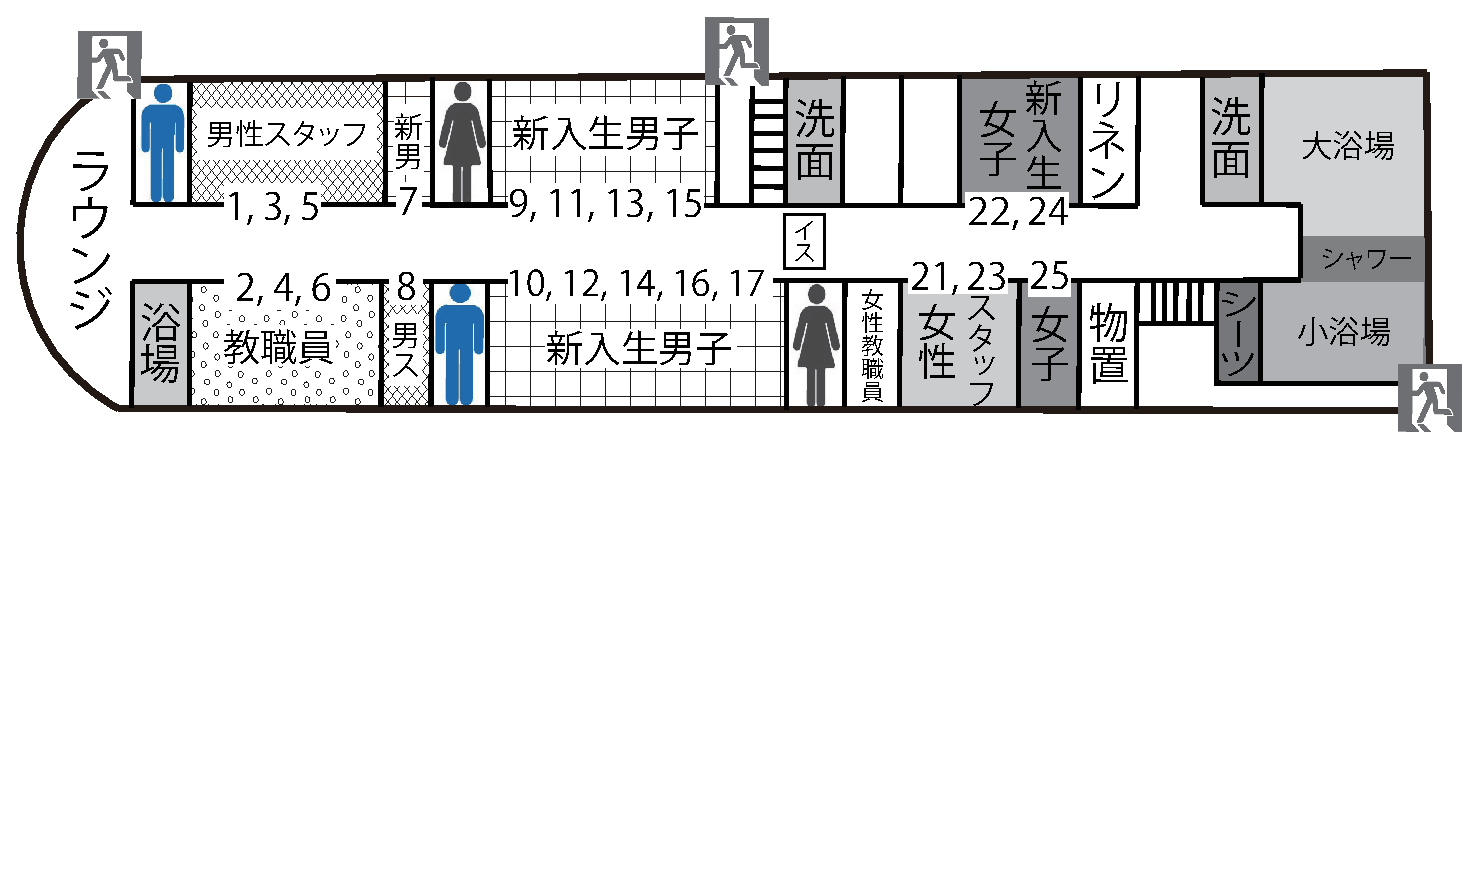
\includegraphics[scale=0.6]{./10/syushin.eps}
\vspace{-45mm}
\caption{就寝部屋割り}
\label{fig:futon_katazuke}
\end{center}
\end{figure}

% 注意事項やスタッフに周知しておくべきことがあれば記入する
\subsection{備考}
\begin{itemize}
%\item 小松(くろしお棟1担当スタッフ),宮尾(くろしお棟3担当スタッフ)は野外炊事から荷物を取りに行く時,第一集会室にいる岡本から指導者棟(龍馬・慎太郎)の鍵をもらう
%\item 基本的に,小松,宮尾が指導者棟の鍵を岡本に返却するまで,スタッフは指導者棟を使用しない
%\item その他,指導者棟の鍵が必要な人は鍵係(岡本)に連絡して鍵をもらう(指導者棟を利用する場合は,適宜報告LINEに連絡する)
%\item 時間や手間の都合上鍵を又貸しする場合は,その旨を報告LINEに報告して誰が鍵をもっているのか明確にしておく
%\item 鍵係は常に連絡がとれる状況にしておく
\item 小松,小島,西森,堀川は、夜の宴終了まじかに入浴しないようにする。
\end{itemize}

% \subsection{連絡事項}
% \begin{table}[h]
% \begin{tabular}{|c|c|c|c|}
% \hline
% {報告者}&{内容}&{タイミング}&{備考}\\ \hline\hline
% Aさん & 指導者棟・慎太郎の浴場使用 & 1回目入浴開始時 & 大浴場で入浴できない新入生がいた場合のみ\\ \hline
% Bさん & 指導者棟・龍馬の浴場使用 & 1回目入浴開始時 & 小浴場で入浴できない新入生がいた場合のみ\\ \hline
% Cさん & くろしお棟1の入浴終了 & 1回目入浴終了時 & \\ \hline
% Dさん & くろしお棟3の入浴終了 & 1回目入浴終了時 & \\ \hline
% Fさん & 指導者棟・慎太郎の浴場使用 & 2回目入浴開始時 & 大浴場で入浴できない新入生がいた場合のみ\\ \hline
% Gさん & くろしお棟2の入浴終了 & 2回目入浴終了時 & \\ \hline
% \end{tabular}
% \label{tab:bath}
% \caption{各棟入浴開始時間}
%\end{table}

%\include{end}
